% !TeX root = ./00.ppgcc-2020.tex

\chapter{Fundamentos Científicos e Tecnológicos}\label{cha:fundamentos}

Este Capítulo aborda conceitos que embasam esse trabalho,
conceitos teóricos de
ambientes e arquiteturas de computação distribuída e detecção de novidade,
e conceitos técnicos, como plataformas de processamento distribuído de fluxo
de dados e o algoritmo MINAS.

\section{Ambientes de Computação Distribuída}

Esta \Section relaciona três ambientes de computação distribuída habitualmente
utilizados para o processamento de dados massivos relacionados a redes de
dispositivos \iot: computação em nuvem, computação de borda, e computação em névoa.
A computação em nuvem (\emph{Cloud Computing}) é
aplicada a vários problemas, e para sistemas \iot 
fornece vastos recursos como computação e armazenamento para onde geralmente os dispositivos
enviam todos dados relevantes ao sistema.
O segundo e terceiro ambientes são computação de borda (\emph{edge computing})
e a computação em névoa (\emph{fog computing}) que utilizam os recursos
computacionais distribuídos presentes em nós localizados entre os dispositivos
de borda e a nuvem com diversas 
intenções, desde privacidade até redução de latência.

% \subsection{Computação em Nuvem}

A computação em nuvem, ou simplesmente nuvem, habilita o acesso através da rede a um grupo compartilhado de
recursos de computação configuráveis, como servidores, redes, aplicações,
armazenamento, etc.
Tais recursos podem ser provisionados ou liberados sob
demanda rapidamente com o mínimo esforço de gerenciamento
e mínima interação com o provedor destes recursos \cite{NIST2011}.

As principais características do ambiente de nuvem, segundo \citeonline{NIST2011}
são: serviço sob demanda, amplo acesso à rede, agrupamento de recursos,
elasticidade e serviço mensurado.
Segundo \citeonline{NIST2011}, a implantação da Computação em Nuvem pode
ocorrer através dos seguintes modelos: privada, comunitária, pública, híbrida.
Das implantações, a pública é a mais comum, sendo gerenciada e operada por um
provedor de nuvem e a infraestrutura é provisionada e oferecida para uso
público.

% \subsection{Computação de Borda}

A computação de borda (\emph{edge computing}) refere-se às
tecnologias que permitem que a computação seja executada na borda da rede.
Define-se borda ou \emph{edge} como qualquer recurso de computação e de rede ao
longo do caminho entre as fontes de dados e os data centers da nuvem
\cite{Shi2016}.
Na borda, é possível fazer armazenamento, processamento e descarregamento de
dados, assim como distribuir as requisições e entregar os serviços das nuvens
aos usuários.
\citeonline{Shi2016} ressalta que essas capacidades (dentre outras) dos nós da
borda (\emph{edge nodes}) possibilitam que a computação de borda reduza a
latência na resposta da nuvem, pré-processando os dados nos nós da borda,
aproveitando melhor a banda e a transmissão de dados, e também consumindo menos
recursos de computação na nuvem.
Além disso, o autor ainda acrescenta que a computação de borda pode aumentar a
privacidade dos dados, uma vez que eles podem ser processados no próprio
dispositivo final.

A computação de borda tenta trazer a computação mais próxima das fontes de
dados.
Os componentes desse tipo de computação podem ser
tanto produtores como consumidores, não só requisitando serviços e conteúdo da
nuvem, mas também realizando tarefas da nuvem.
Algumas aplicações da computação de borda incluem: análise de vídeo;
em sistemas críticos para redução de latência;
descarregar a nuvem de parte da computação;
privacidade dos dados produzidos, mantendo-os fora de ambientes públicos;
redução das cargas de dados na rede e
processamento distribuído de sensoriamento massivo em cidades inteligentes \cite{Shi2016}.

% \subsection{Computação em Névoa}

\citeonline{Dastjerdi2016} e \citeonline{IEEECommunicationsSociety2018} \todo{Verificar esta referência}
mencionam que a enorme massa de dados gerados por ambientes IoT pode ser
processada em nuvem, entretanto a latência produzida pela transferência desses
dados para a nuvem e o retorno do resultado pode não ser toleradas por sistemas
críticos que sejam sensíveis a latência como monitoramento de saúde e resposta a
emergências.
\citeonline{IEEECommunicationsSociety2018} ainda acrescenta que enviar tantos
dados à nuvem
para processamento e armazenamento pode ser ineficiente e não escalável, devido à
saturação de dados na rede.
O ambiente de computação de borda foi proposto para trazer o
processamento e armazenamento para os dispositivos de borda tentando solucionar
esses problemas.
Entretanto, dispositivos de borda comumente não podem lidar com várias
aplicações IoT competindo pelos seus recursos limitados, o que poderia causar a
contenção dos recursos e o aumento na latência do processamento
\cite{Dastjerdi2016}. Portanto, para solucionar estas questões de latência e
capacidade limitada dos dispositivos de borda, a computação em névoa foi proposta.

A computação em névoa (\emph{fog computing}) é um paradigma que distribui
as capacidades de computação, armazenamento e rede entre os nós próximos
das fontes dados
e dos dispositivos finais, mas não necessariamente localizados na borda,
dando a esses nós características de uma nuvem
\cite{Bonomi2012,Dastjerdi2016,IEEECommunicationsSociety2018}.
% \todo[inline]{IEEECommunicationsSociety2018 ??  Verificar}
Esse tipo de computação evita a sobrecarga dos dispositivos de borda.

\citeonline{Bonomi2012} e
\citeonline{Dastjerdi2016} consideram computação em névoa como complementar da
computação em borda, podendo a computação em névoa aproveitar os recursos da
nuvem e da borda.
\citeonline{IEEECommunicationsSociety2018} considera que a
principal diferença entre esses dois tipos de computação está no número de
camadas.
Enquanto computação de borda tem
camadas menores, pois atua só nos
dispositivos de borda, computação em névoa tem mais camadas e um modelo
hierárquico, pois não atua só na camada de borda.

Segundo \citeonline{Bonomi2012} e \citeonline{Dastjerdi2016}, as principais
características da computação em névoa são:

\begin{itemize}

    \item \textbf{Mobilidade:} é essencial que as aplicações para computação em névoa sejam
    capazes de se comunicar com dispositivos móveis, por exemplo, utilizando
    protocolos que considerem a mobilidade dos nós;

    \item \textbf{Heterogeneidade:} os nós nesse tipo de paradigma possuem
    configurações e formatos diferentes e podem estar implantados em ambientes
    distintos;

    \item \textbf{Baixa Latência:} \hlhl{computação em névoa} foi proposta para
    atender aplicações que requeiram baixa latência (monitoramento de saúde,
    jogos, realidade aumentada, etc.);

    \item \textbf{Distribuição geográfica:} computação em névoa pode possuir
    milhares de sensores e dispositivos distribuídos geograficamente, com
    consciência de suas localizações (\emph{location awareness});

    \item \textbf{Alto número de nós:} seguindo os ambientes IoT, a computação
    em névoa pode ser composta por milhares de nós;

    \item \textbf{Interoperabilidade e federação:} os componentes da computação
    em névoa devem ser capazes de interoperar, e o serviços devem ser federados
    \hlhl{ao longo de diferentes domínios};

    \item \textbf{Uso de fluxo de dados e aplicações em tempo real:} a
    computação em névoa pode envolver aplicações que processam em lote, mas na
    maior parte das vezes envolve aplicações com requisito de processamento em
    tempo real, e para isso fazem o uso de fluxo de dados. Por exemplo, os
    sensores de um rede IoT escrevem a informação no fluxo de dados, a
    informação é processada, ações são inferidas e traduzidos em
    ações nos componentes atuadores.

\end{itemize}

Algumas aplicações para computação em névoa são:
cidades inteligentes e
semáforos inteligentes que enviam sinais de alerta aos veículos e coordenam os
sinais verdes com outros semáforos através de sensores (veículos, pedestres,
ciclistas);
na área de saúde, para monitorar e prever situações de pacientes que
estão conectados a sensores;
em prédios inteligentes, que são dotados de sensores
de umidade, temperatura, qualidade do ar, ocupação, sendo que a partir das
informações deles, é possível alertar os ocupantes do prédio em algum caso de
emergência.

\section{Arquiteturas e Plataformas de Processamento de Fluxos de Dados}
\label{sec:frameworks}

\todo[inline]{Me parece que Spark, Flink ... são ambientes, enquanto Cloud e Fog estão mais para plataformas (seção 2.1). }
Tradicionalmente, aplicações
foram construídas com um sistema gerenciador de
banco de dados relacional ou não-relacional associado.
Essa arquitetura,
nomeada de ``arquitetura totalmente incremental'' por \citeonline{marz2015big},
foi evoluída e simplificada iterativamente durante décadas de uso, porém ela não
é adequada para sistemas em tempo real, como os sistema de fluxo de dados.
O volume e a velocidade de dados em um fluxo de dados leva à necessidade de
distribuir o processamento, acrescentando poder computacional a cada nó
adicionado.
Entretanto, desafios como comunicação eficiente e sincronização de estado
entre os nós, assim como tolerância a falhas, aumentam a complexidade de
construção de um sistema distribuído em relação a um sistema tradicional.

\newcommand{\lambdaa}{\xspace\emph{Lambda}\xspace}
\newcommand{\kappaa}{\xspace\emph{Kappa}\xspace}

Para mitigar problemas associados à construção de sistemas \emph{Big Data} e de
fluxos de dados, arquiteturas de processamento de fluxo de dados distribuído
foram propostas, como a arquitetura \lambdaa \cite{marz2015big} e \kappaa
\cite{Kreps2014}, além de diversas plataformas, tanto de \emph{Big Data} com
características de tempo real, como especializadas em fluxo de dados.

\emph{MapReduce} é a primeira plataforma de processamento de conjuntos massivos
de dados que atingiu uso generalizado.
Nessa implementação, uma biblioteca gerencia a distribuição, paralelização,
tolerância a falhas e balanceamento de carga.
Ao usuário da biblioteca resta implementar duas funções:
\emph{Map}, que recebe um par ordenado
$(chave, valor)$ e emite um conjunto de pares intermediários na mesma estrutura;
\emph{Reduce}, que recebe uma chave e um conjunto de valores gerado pelo agrupamento
de pares com essa mesma chave \cite{Dean2004}.

Em prática, um \emph{cluster MapReduce} tem centenas de processadores e o
conjunto de dados é armazenado em um sistema de arquivos distribuído que é lido
pela plataforma com programas escritos por usuários sendo executados sob
supervisão de um nó mestre.
Essa implementação tem esquema geral de processamento em lotes que não atende o
requisito de baixa latência.
\nobreakdash \emph{MapReduce} é uma das principais influências na criação da arquitetura \lambdaa \cite{marz2015big}.

\emph{Apache Hadoop} é uma coleção de ferramentas, incluindo: \emph{Hadoop
Distributed File System} (HDFS, um sistema de arquivos distribuído), \emph{Hadoop
YARN} um gerenciador de recursos em cluster e escalonador de trabalhos e,
\emph{Hadoop MapReduce}, um sistema baseado em \emph{YARN}, implementando o modelo
\emph{MapReduce} \cite{ApacheHadoop2020}.

\emph{Apache Spark}, analogamente ao \emph{Hadoop}, é um \emph{framework} para
construção de sistemas de computação distribuída em \emph{cluster}, com garantias
de tolerância a falhas.
No entanto, o modelo de processamento diverge
significativamente do tradicional \emph{MapReduce}, utilizando em lugar do HDFS
um multiconjunto imutável distribuído (\emph{Resilient Distributed Dataset}
- RDD) com um escalonador de trabalhos representados por grafos acíclicos
direcionados (\emph{directed acyclic graph} - DAG), otimizador de consultas e
motor de execução \cite{ApacheSpark2020}.

Uma das extensões de \emph{Apache Spark} é o \emph{Spark Streaming}, que é um
sistema de processamento de fluxo de dados 
escalável e tolerante a falhas
\cite{zaharia2016,sparkStreaming2016}.
\emph{Spark Streaming} implementa processamento incremental de fluxo de
dados usando o modelo de fluxos discretizados em que dividem-se os dados de entrada
em micro-lotes (ex: a cada 100 milissegundos) e combinam-se regularmente com o
estado nos RDDs para produzir novos resultados \cite{zaharia2016}.
Essa estratégia traz benefícios sobre os sistemas de fluxos de dados distribuídos
tradicionais, pois permite a consistência e recuperação de falhas rapidamente,
devido à \notahl{?}\hlhl{linhagem de RDD} (\emph{RDD lineage})
e à combinação do fluxo de dados com
consultas em lotes e interativas \cite{sparkStreaming2016,Lopez2018}.

\emph{Apache Storm} é um sistema de computação tolerante a falhas em tempo
real que \notahl{quem disse?!}\hlhl{facilita o processamento} de fluxo de dados
\cite{ApacheStorm2020,Lopez2018}.
Ao invés de executar trabalhos (\emph{jobs}) como algumas ferramentas citadas
anteriormente, \emph{Apache Storm} \notahl{?}\hlhl{executa topologias}.
Os \emph{jobs} eventualmente finalizam, e as topologias executam continuamente até
serem finalizadas manualmente.
Uma topologia constitui-se de processos trabalhadores (\emph{workers}) sendo executados
em um \emph{cluster} de nós que são gerenciados pelo nó mestre que além de
coordenar e distribuir execução, monitora falhas.
Uma topologia pode ser representada por um grafo de computação direcionado
acíclico (DAG).

O \emph{Apache Flink} é uma plataforma de processamento distribuído para
computação com estado gerenciado (\emph{stateful}) sobre fluxo de dados limitados (têm início e
fim) e ilimitados (não têm fim definido) \cite{ApacheFlink2020}.
Essa plataforma segue um paradigma que abrange o processamento de fluxos de
dados contínuos e o processamento em lote \cite{Carbone2015,Lopez2018}.
O \emph{Apache Flink} pode ser integrado a vários gerenciadores de \emph{cluster}
comuns, como \emph{Hadoop Yarn}, \emph{Apache Mesos}, e \emph{Kubernetes}, mas também pode ser
configurado para ser executado como um \emph{cluster stand-alone}.
Já o acesso programático a essa plataforma pode ser feito através das linguagens
Java, Scala ou Python.

\section{Interface de Troca de Mensagens}
\todo[]{}
% \todo[inline]{Não é usual traduzir MPI e nem SPMD. Ambos são bem conhecidos na comunidade.}
Em um sistema distribuído multiprocessado, a memória é distribuída entre
múltiplos nós e processos, tendo cada processo acesso direto somente a sua memória
local.
Para esse tipo de sistema, o paradigma de programação paralela \spmd onde
múltiplas instâncias de um único programa tratam parcelas de dados, pode ser
implementado utilizando o conceito de memória distribuída compartilhada através
de troca de mensagens.
Nesse modelo, cada
processo tem sua memória local e se comunica com outros processos através da
troca de mensagens \cite{mpi-book}.
Observando boas práticas e melhores funcionalidades ao longo dos anos, a
comunidade e a indústria padronizaram esse modelo de troca de mensagens no
padrão \acf{MPI}.

O \mpi\footnote{Disponível em \url{https://www.mpi-forum.org/}.} é um padrão que
estabelece um protocolo de comunicação e define sintaxe e semântica para
bibliotecas de troca de mensagens em ambientes de memória distribuída compartilhada.
Esse modelo pode ser implementado desde computadores multiprocessados de memória
compartilhada até supercomputadores com centenas de nós e milhares de
processadores.
O \mpi, por meio de alguma
implementação como OpenMPI e MPICH, permite a construção de um sistema
distribuído com um executável único (monólito) e sua execução em um ambiente gerenciado.

O \mpi tem duas primitivas básicas para comunicação dos processos que são o
enviar (\emph{send}) e o receber (\emph{receive}) \cite{mpi-book}. A primitiva de
envio é composta pelos argumentos: conteúdo da mensagem, tamanho da mensagem,
processo destino, e \emph{tag} para diferenciar mensagens (ex: ordem e conteúdo).
Associado à cada primitiva enviar, a primitiva receber possui os argumentos:
conteúdo da mensagem, tamanho máximo da mensagem, remetente da mensagem, tamanho
real da mensagem, e \emph{tag}.
Além de operações de envio e recebimento, pode-se fazer
envio de mensagens de uma fonte para múltiplos destinos, e um destino receber de
múltiplas fontes numa única operação.

Um dos detalhes importantes quando se utiliza o \mpi com o TCP/IP, é que as
garantias de envio são fornecidas pelo protocolo TCP, ou seja, feito um envio
com a operação \emph{send} o processo que enviou é desbloqueado logo após que a
mensagem é escrita no buffer de saída do TCP do sistema operacional. Portanto,
existe tempo de voo (\emph{time of flight}) entre o envio e recebimento.

O \mpi possui um ambiente de execução e gerenciamento chamado \emph{mpirun} que
recebe como entrada a configuração do cluster e o programa a ser executado, e se
encarrega de iniciar os processos em todos os nós, geralmente por \emph{ssh},
repassando os parâmetros que recebeu a cada processo e o identificador do
processo para que ele saiba qual dado ler e qual função executar sob o paradigma
\spmd.

Este trabalho utiliza o OpenMPI\footnote{Disponível em \url{https://www.open-mpi.org/}.}, que é uma implementação livre de \mpi, para a
comunicação entre os processos de cada nó do cluster.
Cada nó do cluster possui um conjunto de processos, e cada processo possui seu
espaço de endereçamento e é \emph{multithread}, onde as \emph{threads} se comunicam
através da memória compartilhada.
O OpenMPI permite a comunicação entre os processos independente se estão ou não
no mesmo nó.

% \begin{figure}[htb]
%   \centerline{
%     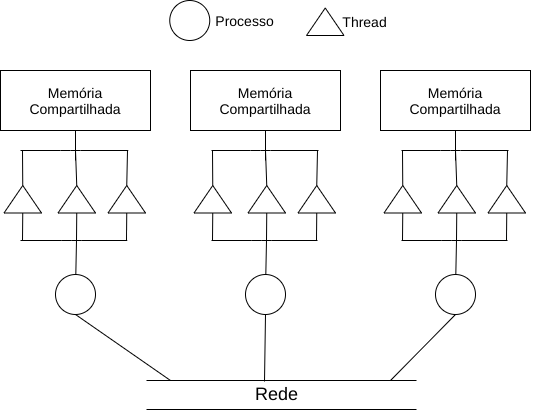
\includegraphics[width=0.55\linewidth,page=1]{figures/mpi-modelo-iot.png}
%   }
%   \caption{Modelo de processos do \mfog.}
%   \label{fig:mpi-modelo}
% \end{figure}

% \todo[inline]{A figura se refere a alfo específico do M-FOG ou algo geral para
% MPI? Se for o primeiro caso, seria melhor colocá-la junto ao texto que apresenta
% o M-FOG. Nesta seção o foco é descrever o MPI.}
O amplo uso de \mpi para programação paralela e distribuída está principalmente pautado no
desempenho. Processadores modernos possuem memórias hierárquicas que beneficiam
programas que fazem o melhor uso de cache. O modelo de passagem de mensagens
permite o particionamento dos dados em fatias menores otimizando o uso de cache
nesses processadores. Portanto, para aplicações limitados por memória pode haver
acelerações super-lineares (\emph{superlinear speedup}) \cite{mpi-book}.

Apesar do \mpi não ter sido idealizado para o processamento de fluxo de dados, ele
permite o controle sobre a distribuição de tarefas de maneira
semelhante ao Apache Flink, porém dispensando o uso de um
gerenciador. Essa dispensa de gerenciador em experimentos preliminares mostrou
crucial para implementação do \mfog em dispositivos IoT, pois não excede o limite de
memória do nó.

Em resumo, o \mpi é utilizado em um programa monólito escrito em C, executado
por múltiplos processos em múltiplos nós, cada processo recebe um conjunto de
dados diferente e, de acordo com o tipo de dado recebido, o processo executa
funções diferentes.
Em adição, os processos podem trocar informações entre si com mensagens,
efetivamente compartilhando segmentos discretos de memória.
Uma das estratégias é a leitura e distribuição de dados por um processo enquanto
os outros processam, dividindo o trabalho, sendo possível desta maneira tratar
de fluxos contínuos de dados de maneira escalável.
% Se for um processo raiz, ele lê e distribui os dados de entrada entre os nós
% folha. Já os nós folha executam todo cálculo de distância e detecção de
% novidades, portanto execução de forma paralela e distribuída.

% \todo[inline]{O ultimo paragrafo mistura MPI com a descrição de como foi
% implementado o M-FOG. Acho que esta seção deveria falar somente do MPI de forma
% genérica: O que é, para que serve e por que foi escolhido para este trabalho.}
